\chapter[Our Framework at Work on the iTrust SWaT System]{Our Framework at Work: Reverse Engineering of the iTrust SWaT System}
\label{application}
\linenumbers

\lettrine{I}{n this} chapter, our main objective is to apply the framework and methodology introduced in Chapter \ref{chap:proposal} to the case study of the iTrust SWaT system, as illustrated in Chapter \ref{casestudy}. The purpose of this analysis is to assess the effectiveness and potential of the proposed framework within the context of a system that closely replicates a real-world water treatment plant, albeit on a smaller scale.

\bigskip
Due to the complexity of the system and the limited space available in this thesis, we will not conduct a comprehensive analysis and reverse engineering of the entire system. Instead, we will focus on specific parts for analysis. We leave it to the reader or those interested in utilizing the proposed methodology and framework to complete the analysis, should they choose to do so.\newline
By focusing on selective components and leaving room for further exploration, we strike a balance between providing valuable insights and acknowledging the potential for additional research. This approach empowers the reader and interested individuals to explore the iTrust SWaT system further and leverage the proposed methodology and framework for a more comprehensive analysis.

\section{Preliminary Operations}
\label{sec:6_preliminar_operations}
Prior to beginning the actual analysis, several preliminary manual operations need to be conducted on the physical process dataset utilized as a case study, specifically the SWaT system dataset for the year 2015 as outlined in Section \ref{subsec:5_2015_datasets}. To simulate the data-capture process performed by Ceccato et al. using their scanning tool, the original dataset in XLSX format (proprietary to Microsoft Excel) was divided into multiple datasets in CSV format. Each of these datasets corresponds to the individual stages of the SWaT system and contains the respective registers. These resulting files were then saved in the directory specified by the \texttt{raw\_dataset\_directory} directive in the framework configuration file, \textit{config.ini}, ready to be used in the pre-processing phase.\newline
Furthermore, the headers were manually renamed by adding a prefix from \texttt{P1\_} to \texttt{P6\_} to each register's name. This prefix indicates the stages, ensuring that each register is easily identifiable and linked to its corresponding stage.

\section{Planning the Analysis Strategy}
\label{sec:6_analysis_strategy}
The complexity of the system being analyzed necessitates the adoption of a deliberate strategy for the analysis. It is not feasible to rely on trial and error or attempt every possible combination between stages. The former approach may overlook crucial relationships between PLCs or between registers, while the latter may result in excessive and unproductive efforts if the specific portion of the system being analyzed lacks significant information or relationships. \newline
A sound analysis strategy helps us focus on the important parts of the system, improving the quality of the analysis and leading to better process comprehension. By prioritizing our attention, we can gain a deeper understanding of the crucial components, resulting in more informed decision-making and a comprehensive understanding of the overall processes.

\bigskip
To define this strategy, a potential starting point could involve analyzing network traffic to determine the communication patterns and participants within the system. This can be accomplished by utilizing the techniques discussed in Section \ref{subsec:4_network_analysis} on Network Analysis. By applying the Python script described in that section to the data extracted from the network traffic dataset debated in Section \ref{par:5_2015_net_dataset}, we can generate a (simplified) network graph, as illustrated in Figure \ref{fig:6_network_SWaT}.

\begin{figure}[ht]
	\centering
	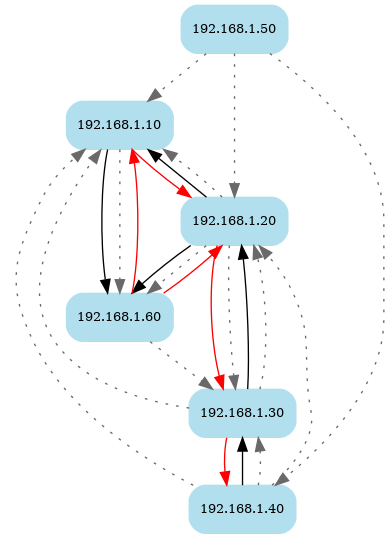
\includegraphics[scale=0.65]{chap6/network2.png}
	\caption{Simplified graph of the iTrust SWaT system network}
	\label{fig:6_network_SWaT}
\end{figure}

The graph clearly illustrates the structure of communications between the PLCs. Referring back to Table \ref{table:5_swat_ip_addresses}, which displays the IP address - PLC associations, we can observe that PLCs 1 through 4 communicate directly and sequentially with each other in a Request/Response communication pattern (represented by red and black arrows, respectively). Additionally, PLC6 communicates with both PLC1 and PLC2. On the other hand, the gray dotted arrows indicate communications for which we have knowledge of a response, but the corresponding request is unknown. For the purposes of our analysis strategy, we will not consider these communications within this context.

\bigskip
Based on our observations, the analysis strategy we will adopt involves considering sequential pairs of PLCs to effectively capture the relationships and implications between registers. Therefore, the PLC pairs we will focus on are PLC1-2, PLC2-3, and PLC3-4. 

\section{Reverse Engineering of the iTrust SWaT System}
\label{sec:6_reverse_SWaT}
Before we delve into the analysis, it is important to provide some preliminary remarks. 

\bigskip
Firstly, the analysis will be structured as a schematic analysis due to space constraints, which prevent us from presenting the extensive inferences and reasoning regarding the system in full detail. However, the general procedure of the methodology and how to reason about the data obtained from the framework have already been demonstrated through examples on the PLC1 of the SWaT system in Chapter \ref{chap:proposal}. We encourage readers to refer to those examples for a more comprehensive understanding. In this analysis, our focus will be on illustrating the conjectures and properties that arise from the analysis, utilizing tables and the outputs generated during the analysis.

\bigskip
The second premise addresses the process of defining the subsystems to be analyzed, which were obtained during the pre-processing phase, during the merge phase of the individual datasets. Apart from the projection determined by the considered PLCs, a time-based selection of the analysis period has also been performed (see Section \ref{subsubsec:4_select_subsystem}). This selection spans a duration of 20,000 seconds, which is equivalent to approximately five and a half hours or roughly five system cycles. The analysis begins at 100,000 seconds, which corresponds to approximately 27 hours from the start of the available data. This deliberate selection aims to exclude the initial transient period during which the SWaT system is initialized. We believe that this time range is more than sufficient for accurately defining the characteristics of the SWaT system components.

\bigskip
The third premise introduces some conventions regarding the PLC registers that will be utilized during the analysis. These conventions aid in identifying the nature and function of the registers. Specifically:

\begin{enumerate}
	\item Registers containing discrete values, such as binary or ternary values, are likely to represent actuators.
	
	\item Registers with continuous values are identified as measurements.
	
	\item Actuators with three states are recognized as valves, while those with two states are considered pumps.
	
	\item Measurements with a wide range between the maximum and minimum values are identified as level sensors for tanks. Sensors with a narrow range may represent other types of measurements such as flow or pressure sensors.
	
	\item Registers with a single constant value are recognized as either relative setpoints or backup actuators. The distinction is made based on the value contained in the register. Binary values or values corresponding to the states of the main actuators indicate backup actuators, while different values (e.g., 20, 40, 80, etc.) suggest the presence of relative setpoints.

	\item Registers with similar names, such as \texttt{P1\_LIT101} and \texttt{P3\_LIT301}, or \texttt{P2\_MV201} and \texttt{P3\_MV302}, indicate the same type of register, such as a valve, pump, level sensor, or other category.
\end{enumerate}

By following these conventions, it becomes easier to interpret and analyze the functionality of the PLC registers within the system.

\subsection{Reverse Engineering of PLC1 and PLC2}
\label{subsec:6_P1P2_analysis}
The initial focus of analysis will be on the pair comprising PLC1 and PLC2. Let's delve into the main features of this subsystem by examining the outcomes obtained from applying the framework to it.

\subsubsection{Pre-processing - Preliminary Analysis}
\label{subsubsec:6_P1P2_preprocessing}

\paragraph{Measurements and Actuators Recognition} 
\label{par:6_P1P2_measures_actuators_recognition}
Listing \ref{lst:6_preproc_P1P2} shows the outcomes obtained from automatic recognition of likely measurements and actuators:

\begin{lstlisting}[language=bash, numbers=left, caption=Preliminary analysis outcomes for sensors and actuators of \texttt{PLC1-2}, label=lst:6_preproc_P1P2]
	Actuators: 
	P1_MV101 [0.0, 1.0, 2.0]
	P1_P101 [1.0, 2.0]
	P2_MV201 [0.0, 1.0, 2.0]
	P2_P203 [1.0, 2.0]
	P2_P205 [1.0, 2.0]
	
	Sensors: 
	P1_FIT101 {'max_lvl': 2.7, 'min_lvl': 0.0}
	P1_LIT101 {'max_lvl': 815.1, 'min_lvl': 489.6}
	P2_AIT201 {'max_lvl': 256.5, 'min_lvl': 252.9}
	P2_AIT202 {'max_lvl': 8.4, 'min_lvl': 8.3}
	P2_AIT203 {'max_lvl': 342.8, 'min_lvl': 320.0}
	P2_FIT201 {'max_lvl': 2.5, 'min_lvl': 0.0}
	
	Hardcoded setpoints or spare actuators: 
	P1_P102 [1.0]
	P2_P201 [1.0]
	P2_P202 [1.0]
	P2_P204 [1.0]
	P2_P206 [1.0]
\end{lstlisting}

Based on the results shown in Listing \ref{lst:6_preproc_P1P2}, the framework has recognized \texttt{P1\_MV101}, \texttt{P1\_P101}, \texttt{P2\_MV201}, \texttt{P2\_P203}, and \texttt{P2\_P205} as \textbf{likely actuators}. The actuators indicated by the \textit{Pxxx} string are binary actuators, meaning they have two states represented by the values 1 and 2. On the other hand, the actuators identified by the \textit{MVxxx} string are ternary actuators with three distinct states: 0, 1, and 2. According to the third premise of Section \ref{sec:6_reverse_SWaT}, for point 3, actuators denoted by the \textit{Pxxx} string will be classified as \textbf{pumps}, while those labeled with \textit{MVxxx} will be recognized as \textbf{valves}.

\bigskip
\texttt{P1\_FIT101}, \texttt{P1\_LIT101}, \texttt{P2\_AIT201}, \texttt{P2\_AIT202}, \texttt{P2\_AIT203}, and \texttt{P2\_FIT201} have been identified as \textbf{likely measurements}. Each measurement provides a specific range of values, spanning from a maximum to a minimum value. Based on the range of values reported by these measurements and according to the third premise of Section \ref{sec:6_reverse_SWaT}, for point 4, it is reasonable to infer that \texttt{P1\_LIT101} could potentially be a \textbf{level sensor for a tank}.

\bigskip
In addition, there are some registers that have been recognized as \textbf{hardcoded setpoints} or \textbf{spare actuators} due to their constant values. These registers share a resemblance to the previously identified pump registers. According to points 5 and 6 of the third premise in Section \ref{sec:6_reverse_SWaT}, it is reasonable to assume that these registers correspond to \textbf{spare actuators}. Furthermore, the fact that they have a constant value of 1 indicates that they might represent the \textbf{OFF state} of the pumps.

%\noindent Based on the output presented in the listing, we have compiled a preliminary set of conjectures and properties for the subsystem in question. These findings are summarized in Table \ref{table:6_p1p2_actuators_1}:

%{	\small
%	\begin{longtable}[l]{p{0.01\textwidth} p{0.45\textwidth} p{0.46\textwidth}}
%		\hline
%		\textbf{\#} & \textbf{Conjecture / Property} & \textbf{Reason} \\
%		\hline
		
%		1 & \texttt{P1\_LIT101}, \texttt{P1\_FIT101}, \texttt{P2\_FIT201}, \texttt{P2\_AIT201}, \texttt{P2\_AIT202}, \texttt{P2\_AIT203} are \textbf{measurements}. & Registers contain continuous numerical values.\\
%		\hline
		
%		2 & \texttt{P1\_LIT101} is identified as the \textbf{level sensor} specifically associated with a \textbf{tank} & Sensor has a wide range of values (minimum 489, maximum value of 815).\\
%		\hline
		
%		3 & \texttt{P1\_MV101}, \texttt{P1\_P101}, \texttt{P2\_MV201}, \texttt{P2\_P203} and \texttt{P2\_P205} are \textbf{actuators}. & Registers contain discrete numerical values.\\
%		\hline
		
%		4 & \texttt{P1\_MV101} and \texttt{P2\_MV201} assume three distinct states, represented by the values 0, 1, and 2. They can be identified as \textbf{valves}.& Obvious from the output and from point 3 of the third premise in Section \ref{sec:6_reverse_SWaT}\\
%		\hline
		
%		5 & \texttt{P1\_P101}, \texttt{P2\_P203} and \texttt{P2\_P205} assume two distinct states, represented by the values 1, and 2. They can be identified as \textbf{pumps}. & Obvious from the output and from point 3 of the third premise in Section \ref{sec:6_reverse_SWaT}\\
%		\hline
		
%		6 & \texttt{P1\_102}, \texttt{P2\_P201}, \texttt{P2\_P202}, \texttt{P2\_P204} and \texttt{P2\_P206} are \textbf{spare actuators}. & Registers contain constant numerical values.\\
%		\hline 
		
%		7 & A spare actuator in state 1 is considered to be \textbf{OFF}. & Assumption on the actuator states.\\
%		\hline
		
%		\caption{Likely measurements and actuators conjectures for PLC1-2}
%		\label{table:6_p1p2_actuators_1}
%	\end{longtable}
%}

\paragraph{Actuator State Durations}
\label{par:6_P1P2_actuators_duration}
To gain a deeper understanding of the different states (0, 1, and 2) associated with valves \texttt{P1\_MV101} and \texttt{P2\_MV201}, we can analyze the duration of each state. Listing \ref{lst:6_preproc_P1P2_actuator_duration} provides information regarding the duration (in seconds) of states for these specific actuators:

\begin{lstlisting}[language=bash, numbers=left, caption=Time duration of the states of actuators \texttt{P1\_MV101} and \texttt{P1\_MV201} of PLC1-2, label=lst:6_preproc_P1P2_actuator_duration]
	Actuator state durations:
	P1_MV101 == 0.0
	9  9  10  9  9  10  9  9  10  9
	
	P1_MV101 == 1.0
	1174  1168  1182  1160  1172
	
	P1_MV101 == 2.0
	669  3019  3012  3000  2981
	
	P2_MV201 == 0.0
	8  8  8  9  9  8  9  9  9  9
	
	P2_MV201 == 1.0
	1057  1057  1045  1038  1039
	
	P2_MV201 == 2.0
	120  3135  3144  3127  3109
\end{lstlisting}

\noindent It is evident that the duration of \textbf{state 0 is relatively short}, averaging around 8-10 seconds, while the other states have much longer durations. This observation suggests that state 0 of a valve is a \textbf{transient state}, indicating a transitional phase within the valve cycle. However, without further information, it is currently not possible to determine the specific position of state 0 within the overall valve cycle.

%{\small
%\begin{longtable}[l]{p{0.01\textwidth} p{0.45\textwidth} p{0.46\textwidth}}
%		\hline
%		\textbf{\#} & \textbf{Conjecture / Property} & \textbf{Reason} \\
%		\hline
		
%		8 & The state 0 of a valve is a \textbf{transient state}. & The duration of state 0 is only a few seconds. However, the subsequent states, have a significantly longer duration.\\
%		\hline
		
%	\caption{Conjecture on the state 0 of actuators}
%	\label{table:6_p1p2_mvstate0}
%\end{longtable}
%}

\paragraph{Actuator State Changes}
\label{par:6_preproc_P1P2_actuator_state_changes}
Now that we have identified \texttt{P1\_LIT101} as the supposed tank, we can examine the trend of the tank level as the actuators change state. Listing \ref{lst:6_P1P2_preproc_changestate} provides information on the levels of the tank in correlation with the state changes of the \texttt{P1\_P101} pump:

\begin{lstlisting}[language=bash, numbers=left, caption=P1\_P101 state changes in relation to P1\_LIT101, label=lst:6_P1P2_preproc_changestate]
	P1_LIT101  P1_P101  prev_P1_P101
	 536.0356        1             2
	 533.3272        1             2
	 542.1591        1             2
	 534.8581        1             2
	 540.5890        1             2
	
	P1_LIT101  P1_P101  prev_P1_P101
	 813.0031        2             1
	 813.0031        2             1
	 811.8256        2             1
	 812.7283        2             1
	 813.3171        2             1
\end{lstlisting}

Based on the speculation that state 1 represents the OFF state of the pump and state 2 represents the ON state, we can analyze the data in Listing \ref{lst:6_P1P2_preproc_changestate}. When pump \texttt{P1\_P101} transitions from the ON state to the OFF state, the average level of \texttt{P1\_LIT101} is 535. On the other hand, when \texttt{P1\_P101} goes from the OFF state to the ON state, the average level of \texttt{P1\_LIT101} is 813. These values correspond to the \textbf{minimum and maximum relative setpoints} of \texttt{P1\_P101}, respectively. \newline
Based on this information, we can infer that pump \texttt{P1\_P101} is responsible for \textbf{emptying the tank}. Moreover, it can be extended to assume that a pump, in general, is responsible for \textbf{water outflow}.

\bigskip
Applying the same analysis to the data for valve \texttt{P1\_MV101}, which is not reported for conciseness, we can speculate that \texttt{P1\_MV101} is responsible for \textbf{filling the tank}. In this case, states 1 and 2 would represent the \textbf{OFF and ON states of the valve}, respectively. The relative setpoints of \texttt{P1\_MV101} are approximately 500 (minimum) and 800 (maximum).\newline
By extending this analysis, we can speculate that a valve, such as \texttt{P1\_MV101}, is responsible for controlling the \textbf{water inflow}.


%{	\small
%	\begin{longtable}[l]{p{0.01\textwidth} p{0.45\textwidth} p{0.46\textwidth}}
%		\hline
%		\textbf{\#} & \textbf{Conjecture / Property} & \textbf{Reason} \\
%		\hline
		
%		9 & State 1 of the pump \texttt{P1\_P101} corresponds to the \textbf{OFF state} of the actuator; state 2 of \texttt{P1\_P101} corresponds to the \textbf{ON state} of the actuator. & Derived from Conjecture 7.\\ 
%		\hline
				
%		10 & The \textit{relative setpoints} of \texttt{P1\_P101} are approximately 535 (minimum) when state change to 1 and approximately 813 (maximum) when state change to 2. & Observation derived from output\\
%		\hline
		
%		11 & \texttt{P1\_P101} is responsible for \textbf{emptying the tank} represented by \texttt{P1\_LIT101}. & Derived from Conjecture 9 and 10 \\
%		\hline
		
%		12 & Pumps are responsible for \textbf{water outflow}. & Corollary to Conjecture 11\\
%		\hline		
		
%		13 & State 1 of the valve \texttt{P1\_MV101} corresponds to the \textbf{OFF state} of the actuator; state 2 of \texttt{P1\_MV101} corresponds to the \textbf{ON state} of the actuator. & Derived from Conjecture 7.\\
%		\hline
		
%		14 & The \textit{relative setpoints} of \texttt{P1\_MV101} are approximately 500 (minimum) when state change to 2 and approximately 800 (maximum) when state change to 1. & Observation derived from output\\
%		\hline
		
%		15 & \texttt{P1\_MV101} is responsible for \textbf{filling the tank} represented by \texttt{P1\_LIT101}. & Derived from Conjecture 13 and 14 \\
%		\hline
		
%		16 & Valves are responsible for \textbf{water intake}. & Corollary to Conjecture 15\\
%		\hline

%		\caption{Conjecture on valves and pumps}
%		\label{table:6_p1p2_p101}
%	\end{longtable}
%}

\bigskip
Regarding the elements controlled by PLC2 and the sensor \texttt{P1\_FIT101}, the analysis does not reveal the presence of another tank. Therefore, we cannot determine the exact role of sensors \texttt{P2\_AIT\textit{20x}}, \texttt{P1\_FIT101} and \texttt{P2\_FIT201} at this point.\newline
However, there is a similarity observed between the relative setpoints of \texttt{P1\_P101} and those of \texttt{P2\_MV201}, \texttt{P2\_P203}, and \texttt{P2\_P205}. These registers exhibit very similar values during state changes, suggesting a potential relationship or similar control behavior between them.

\vfill

\subsubsection{Graphs and Statistical Analysis}
\label{subsubsec:6_P1P2_graphs}
Figure \ref{fig:6_P1P2_graph_full} illustrates the graphical representation of the registers in PLC1-2 and their respective trends.

\begin{figure}[ht]
	\centering
	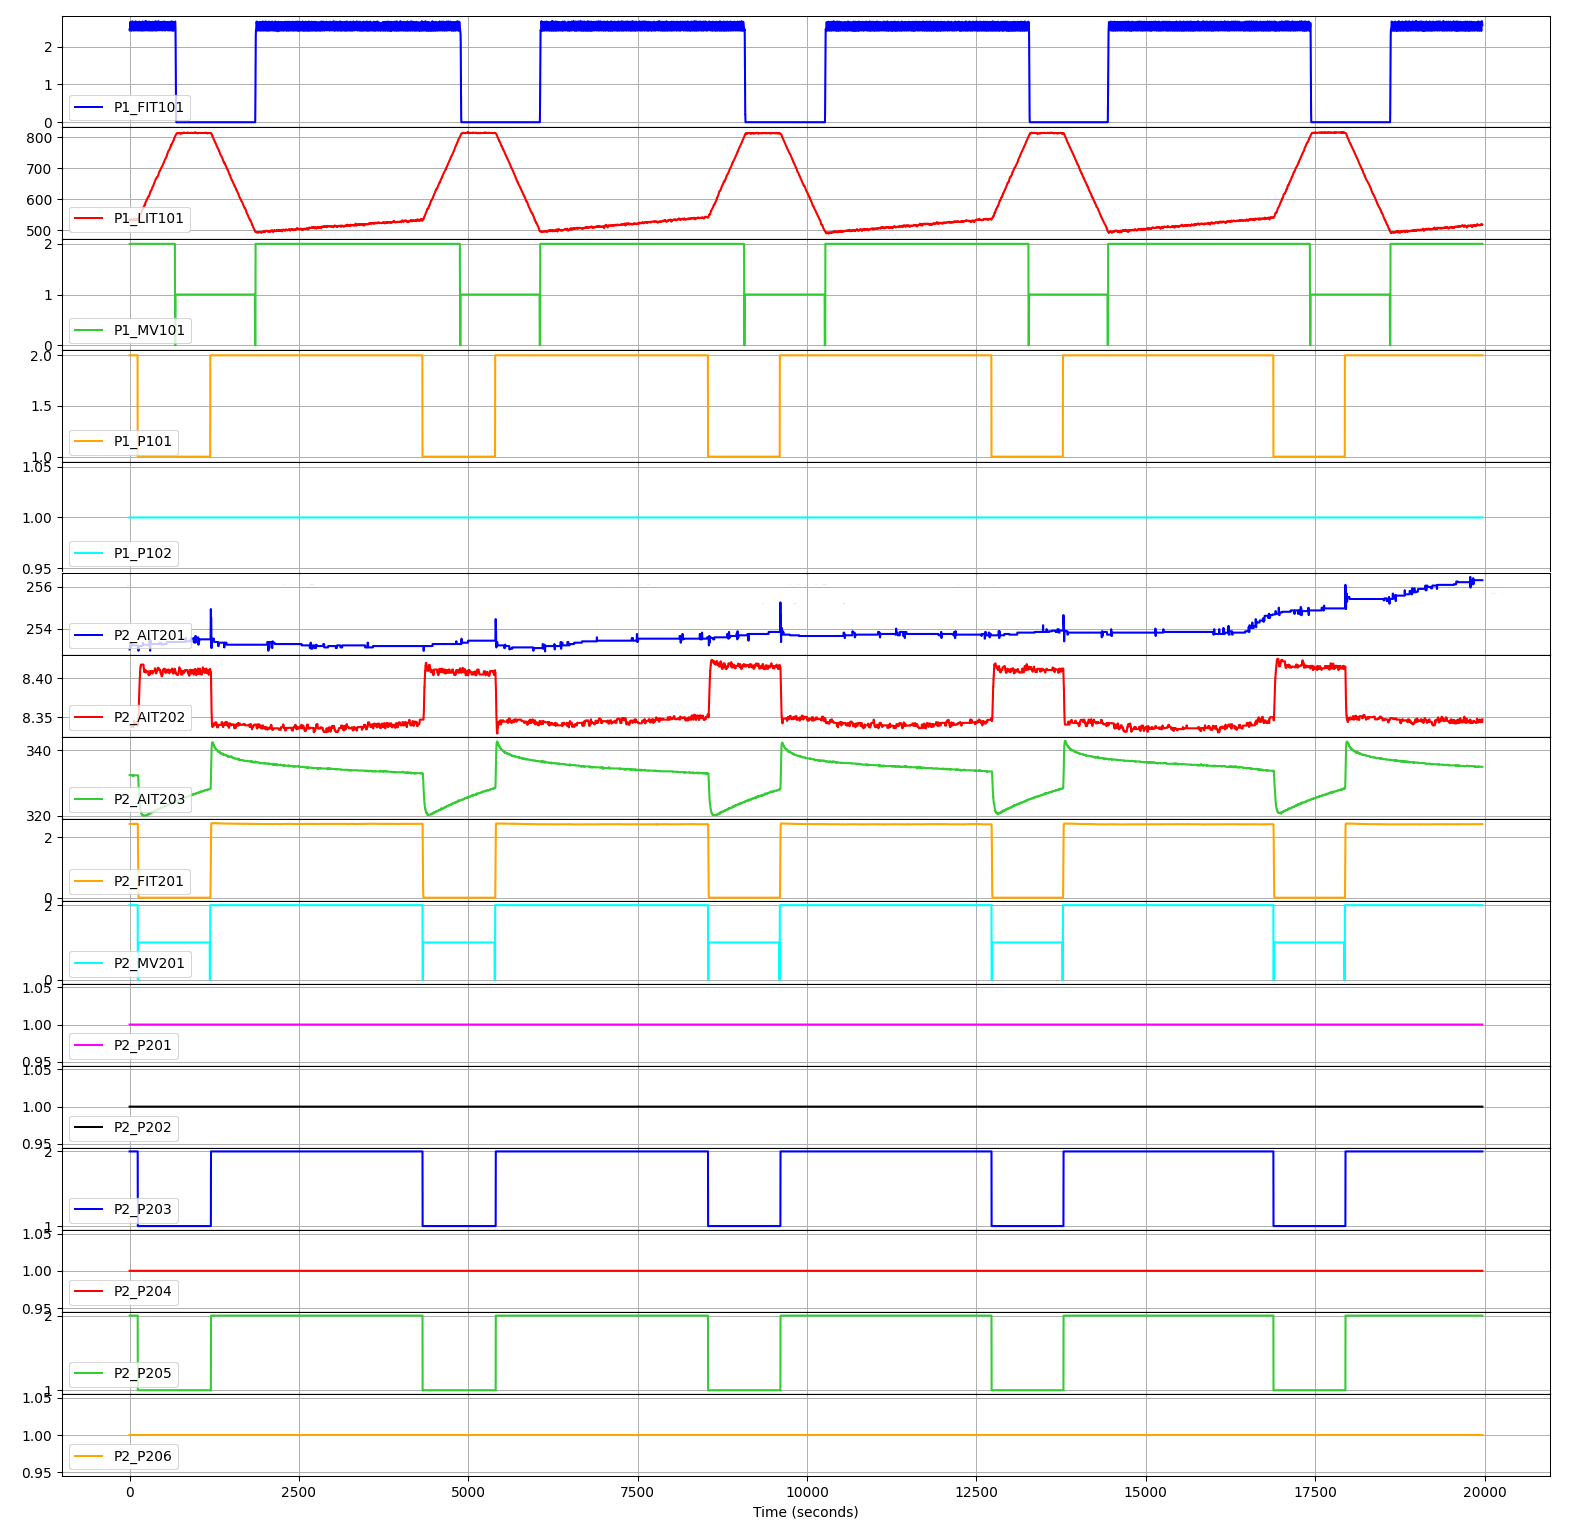
\includegraphics[scale=0.35]{chap6/P1P2_1a.png}
	\caption{Chart of PLC1-2 registers}
	\label{fig:6_P1P2_graph_full}
\end{figure}

The image provides additional support to the conjectures made during the preliminary analysis regarding the spare actuators. Furthermore, it is evident from the graphs that these spare actuators \textbf{do not appear to influence the trend} of any of the measurements. Therefore, based on this observation, we can confidently exclude these registers from further graphical analysis.\newline \newline
Figure \ref{fig:6_P1P2_graph_full_nospare} provides a clearer representation of the subsystem after removing the spare actuators.

\begin{figure}[ht]
	\centering
	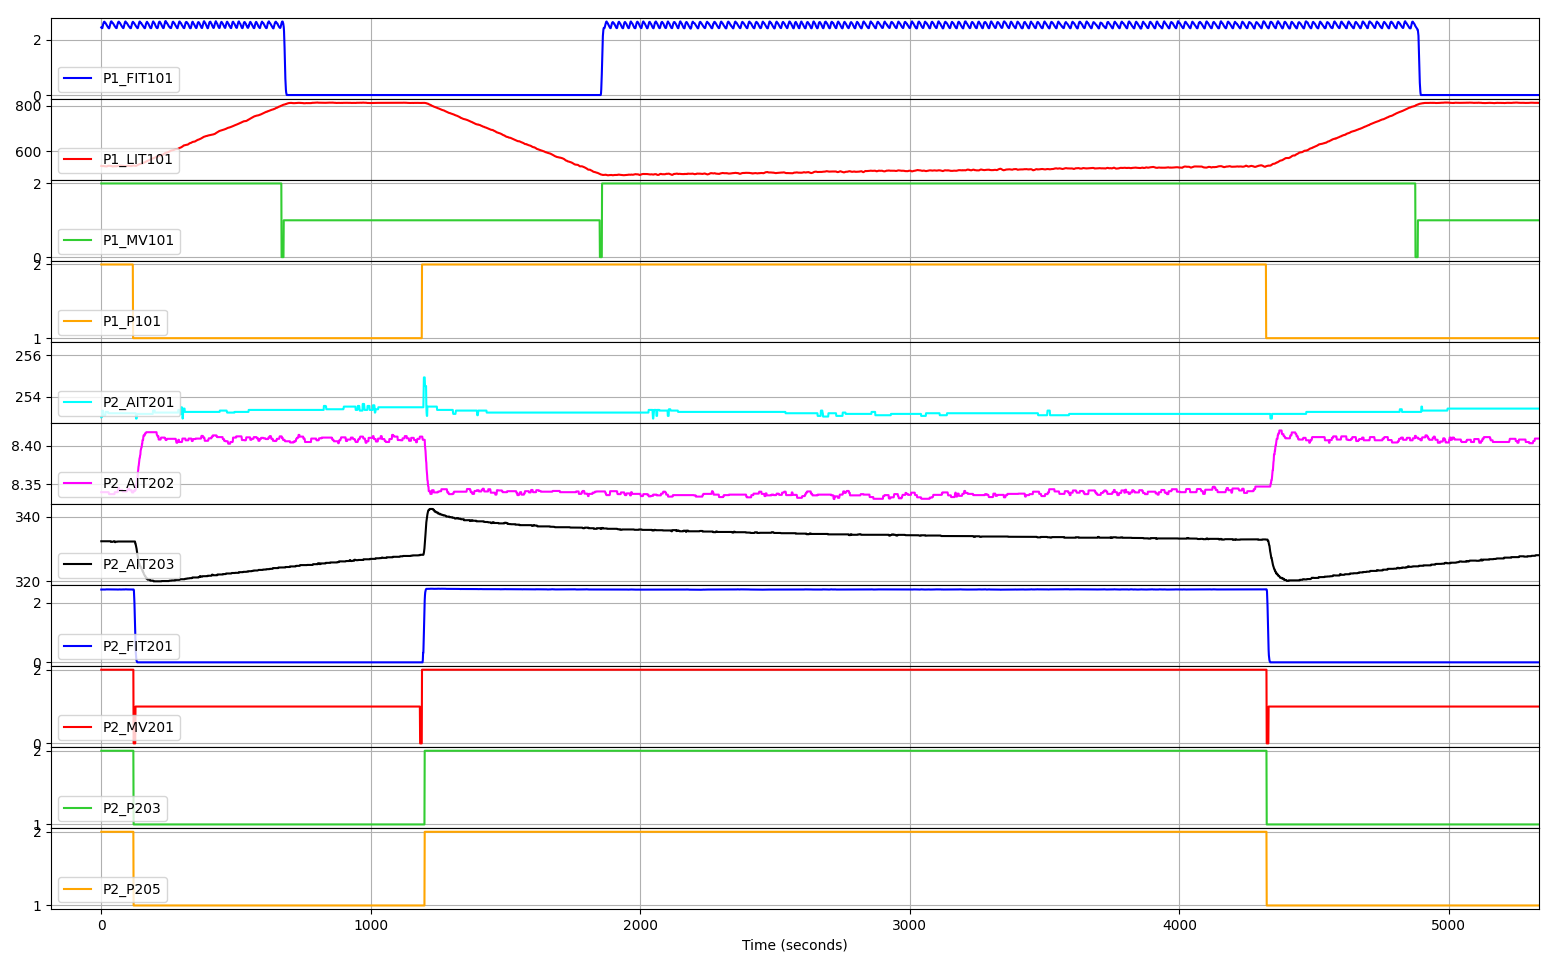
\includegraphics[scale=0.35]{chap6/P1P2_5.png}
	\caption{Chart of PLC1-2 registers without spare actuators (particular)}
	\label{fig:6_P1P2_graph_full_nospare}
\end{figure}

Figure \ref{fig:6_P1P2_graph_full_nospare} provides furthermore additional insights that allow us to speculate on aspects that remained unexplained during the preliminary analysis. Notably, we observe a relationship between \texttt{P1\_FIT101} and the trend of \texttt{P1\_MV101}. When the valve is in the off state, \texttt{P1\_FIT101} registers a value of 0, whereas it registers a value greater than 2 when the valve is open. This suggests that \texttt{P1\_FIT101} could be a \textbf{sensor associated with the flow} of water entering the tank, which is represented by \texttt{P1\_LIT101}. By drawing an analogy with its name, it is plausible to consider \texttt{P2\_FIT201} as another flow sensor.

Altri aspetti interessanti che sono evidenti dal grafico: AIT201 che non segue un andamento ciclico, quindi potrebbe essere un sensore relativo a qualche proprietà dell'acqua. Idem AIT202, a giudicare dal range ristrettissimo di valori. Non posso dire nulla per AIT203. 
MV201 abbiamo detto che è una valvola responsabile dell'inflow, ma qui non ci sono altre taniche apparenti: quindi deve riempire qualcos'altro, a giudicare dalla durata dei suoi stati e dall'andamento. Infine, trovare la relazione tra l'andamento ciclico di AIT202-3 e gli altri attuatori. L'analisi non è ovviamente esaustiva.

%Conjecture 1 and 2, which involve the identification of the tank level sensor and measurements, are confirmed by the charts. Additionally, Conjecture 11 and 12 regarding pump behavior and Conjecture 15 and 16 regarding valve behavior in relation to the tank are also validated. Furthermore, Conjecture 8, which suggests that valves have a 0 state, is also confirmed.\newline
%Looking at the plot, we can make further conjectures based on the observed trends and patterns (Table \ref{table:6_p1p2_graph_conj_1}):

%{	\small
%	\begin{longtable}[l]{p{0.01\textwidth} p{0.45\textwidth} p{0.46\textwidth}}
%		\hline
%		\textbf{\#} & \textbf{Conjecture / Property} & \textbf{Reason} \\
%		\hline
%		17 & The trend of \texttt{P1\_FIT101} follows the trend of \texttt{P1\_MV101} & \texttt{P1\_FIT101} takes a value of 0 when the valve \texttt{P1\_MV101} is OFF, and positive values (> 2) when the valve is ON.\\
%		\hline
		
%		18 & \texttt{P1\_FIT101} is a \textbf{flow sensor} related to the inlet water flow at \texttt{P1\_LIT101}. & Corollary to Conjecture 17\\ 
%		\hline
		
%		19 & \texttt{P2\_FIT201} is also a likely \textbf{flow sensor}. & By analogy with \texttt{P1\_FIT101} (point 6 of the third premise in Section \ref{sec:6_reverse_SWaT})\\ 
%		\hline
		
%		20 & There is a correlation between the trend of \texttt{P1\_P101} and the trend of \texttt{P2\_MV201}. & Observation derived from the plot\\ 
%		\hline
		
%		21 & \texttt{P2\_MV201} is responsible for \textbf{filling a tank} that is \textit{not} part of this subsystem. & Sensors \texttt{P2\_AIT202} and \texttt{P2\_AIT203} do not exhibit an increasing trend when the valve is ON, and there is no apparent correspondence between the trend of the valve and the trend of \texttt{P1\_LIT101}.\\ 
%		\hline
		
%		22 & \texttt{P2\_AIT201} is a sensor that measures \textbf{some property of the water}. & Sensor does not show a cyclic pattern in its measurements.\\
%		\hline
		
%		23 & \texttt{P2\_AIT202} is a sensor that measures \textbf{some property of the water}. & Very narrow range between maximum and minimum values (point 4 of the third premise in Section \ref{sec:6_reverse_SWaT})\\
%		\hline
		
%		24 & The trend of \texttt{P2\_AIT202} and \texttt{P2\_AIT203} follows the trend of \texttt{P2\_P20x} pumps & Observation derived from the plot\\ 
%		\hline
		
%		\caption{Conjecture on the charts}
%		\label{table:6_p1p2_graph_conj_1}
%	\end{longtable}
%}

\bigskip
Currently, the specific role of \texttt{P2\_AIT203} sensors and the correlation between \texttt{P2\_P20x} pumps and \texttt{P2\_AIT202} and \texttt{P2\_AIT203} sensors cannot be determined. These aspects require further analysis and investigation as they exhibit a cyclic pattern that seems to be associated with the behavior of the pumps.

\vfill

\subsubsection{Invariant Inference and Analysis}
\label{subsubsec:6_P1P2_invariants}

\subsubsection{Business Process Analysis}
\label{subsubsec:6_P1P2_bpa}

\subsubsection{Summary}
\label{subsubsec:6_P1P2_summary_table}


\subsection{Reverse Engineering of PLC2 and PLC3}
\label{subsec:6_P2P3_analysis}

\subsubsection{Pre-processing}
\label{subsubsec:6_P2P3_preprocessing}

\subsubsection{Graphs and Statistical Analysis}
\label{subsubsec:6_P2P3_graphs}

\subsubsection{Invariant Inference and Analysis}
\label{subsubsec:6_P2P3_invariants}

\subsubsection{Business Process Analysis}
\label{subsubsec:6_P2P3_bpa}

\subsection{Reverse Engineering of PLC3 and PLC4}
\label{subsec:6_P3P4_analysis}

\subsubsection{Pre-processing}
\label{subsubsec:6_P3P4_preprocessing}

\subsubsection{Graphs and Statistical Analysis}
\label{subsubsec:6_P3P4_graphs}

\subsubsection{Invariant Inference and Analysis}
\label{subsubsec:6_P3P4_invariants}

\subsubsection{Business Process Analysis}
\label{subsubsec:6_P3P4_bpa}

\vfill
\nolinenumbers